\documentclass[11pt,letterpaper]{article}
\usepackage[margin=0.85in]{geometry}
\usepackage[T1]{fontenc}
\usepackage{lmodern}
\usepackage{microtype}
\usepackage{booktabs}
\usepackage{graphicx}
\usepackage{array}
\usepackage{longtable}
\usepackage{xcolor}
\usepackage{hyperref}
\usepackage{fancyhdr}
\hypersetup{colorlinks=true,linkcolor=blue!55!black,urlcolor=blue!55!black,citecolor=blue!55!black}
\graphicspath{{../}}
\setlength{\parskip}{5pt}
\setlength{\parindent}{0pt}
\pagestyle{fancy}
\fancyhf{}
\lhead{Credit Portfolio Analytics}
\rhead{Technical Report}
\cfoot{\thepage}
\setlength{\headheight}{14pt}

\newcommand{\metric}[1]{\textbf{#1}}

\title{From Credit Risk Benchmarking to\ a Portfolio Analyst Tool}
\author{Credit Portfolio Analytics Project}
\date{October 30, 2026}

\begin{document}
\maketitle
\begin{abstract}
This project began as an offline default-prediction exercise and was reshaped into a more recognizable analyst workflow: check a portfolio dataset, make its metrics queryable with SQL, and deliver an interactive monitoring view. It uses the UCI Default of Credit Card Clients data: 30,000 Taiwan credit-card client records from 2005, with six months of repayment history and a next-month default label. A grouped development cross-validation comparison of logistic regression, LightGBM, and XGBoost supports the analytic work; it is not a production model or evidence of current-market performance. The final deliverable includes a local Gradio dashboard backed by DuckDB, reusable SQL, aggregate mart outputs, and a reproducible model-results package.
\end{abstract}
\tableofcontents

\newpage

\section{Executive summary}
The practical question for a portfolio analyst is not only whether a model can rank risk. Analysts also need a repeatable way to validate source data, define metrics, monitor behavior by period and segment, and communicate what the data can and cannot support. This project demonstrates those steps with a public, licensed historical dataset.

The central deliverable is a local Gradio application. It loads the original workbook from a user-selected path, creates an in-memory DuckDB mart, and exposes filtered portfolio counts, historical outcome share, credit-limit summaries, a six-month status-code mix, latest-month code transitions, and segment comparisons. The app does not save the workbook or per-client predictions. The accompanying modeling work shows how a baseline and tree models compare under the same grouped folds.

\begin{itemize}
  \item Source audit: 30,000 rows, 30,000 unique IDs, 23 predictors, no missing cells; target prevalence is 22.12\% in this sample.
  \item Validation: 24,004 development rows in five grouped folds; 5,996 rows reserved as a locked outer test and neither fitted nor scored in the reported comparisons.
  \item Best observed development OOF ranking score among the fixed configurations: LightGBM ROC AUC 0.7829 and average precision 0.5547. XGBoost is close, with AUC 0.7824 and average precision 0.5532.
  \item Feature-family probe: removing the six repayment-status fields lowered LightGBM AUC by 0.0470 and average precision by 0.0946. This is a conditional model ablation, not causal evidence.
  \item No current-portfolio, production, business-value, or deployment claim follows from this old single-vintage dataset.
\end{itemize}

\section{The analyst workflow}
The project is organized as a workflow a credit or business intelligence analyst could recognize:
\begin{enumerate}
  \item \textbf{Inspect the source.} Confirm provenance, license, shape, target, identifiers, missingness, repeated profiles, and code values.
  \item \textbf{Create a trusted analysis boundary.} Exclude identifiers from predictors; group identical predictor profiles so they cannot cross validation partitions; fit preprocessing only on training folds.
  \item \textbf{Compare evidence.} Benchmark a logistic baseline against LightGBM and XGBoost with the same development folds and metrics.
  \item \textbf{Build a queryable mart.} Normalize the six source status fields into client-month records, retain source-code values, and define aggregate queries in DuckDB SQL.
  \item \textbf{Deliver a monitoring view.} Use Gradio controls for age and credit-limit filters and charts/tables that update from parameterized SQL queries.
  \item \textbf{Communicate constraints.} Label the vintage, target timing, segment denominators, and the fact that no operational decision policy has been evaluated.
\end{enumerate}

\section{Data, label, and license}
The source is UCI's \emph{Default of Credit Card Clients} dataset, attributed to I-Cheng Yeh (2009), DOI \href{https://doi.org/10.24432/C55S3H}{10.24432/C55S3H}. UCI lists the dataset under CC BY 4.0. Its current dataset page describes 30,000 records and 23 features, a Taiwan default-payment study, the April--September 2005 payment-history window, and a binary default-payment target. The workbook is kept outside the repository and is read in place.

The prediction label is the literal source column `default payment next month'. The population is existing credit-card clients, not new loan applicants. Status fields map from `PAY\_6' (April 2005) through `PAY\_0' (September 2005); the source field names skip `PAY\_1'. The dashboard groups codes by positive versus non-positive and does not reinterpret the source's ambiguous -2 and 0 values. It calls the views status-code distributions and transitions, not delinquency cure or operational roll rates.

The sample contains 6,636 labeled defaults (22.12\%). This is a cohort statistic, not a current portfolio base rate. Records cover one historical period and lack client-level observation dates suitable for an out-of-time split. Public availability and CC BY attribution do not make this sample representative of a modern lender or a different jurisdiction.

\section{Validation and modeling method}
An outer five-fold `StratifiedGroupKFold' partition with seed 42 sets aside fold 0 (5,996 records) as a locked test. The other 24,004 rows form the development sample. The reported model comparisons use a separate five-fold `StratifiedGroupKFold' design with seed 43. A group is the exact tuple of 23 predictors; `ID' and target are excluded. This prevents repeated profiles from straddling train and validation sets while preserving records whose outcome labels differ.

All reported metrics below pool one out-of-fold probability per development record. The preprocessing and model fit occur within each fold. Logistic regression uses fold-fitted one-hot encoding and standardization. LightGBM uses fold-fitted categorical vocabularies, preserving negative source codes as categories through nonnegative internal category codes. XGBoost uses fold-fitted one-hot encoding. All three are unweighted, fixed configurations; this is not hyperparameter optimization.

\begin{table}[ht]
\centering
\small
\caption{Fixed-model comparison on pooled development out-of-fold predictions (n = 24,004).}
\resizebox{\linewidth}{!}{%
\begin{tabular}{lrrrrrr}
\toprule
Model & ROC AUC $\uparrow$ & Avg. precision $\uparrow$ & Brier $\downarrow$ & Log loss $\downarrow$ & Precision@0.5 & Recall@0.5 \\
\midrule
Logistic regression & 0.7655 & 0.5306 & 0.13745 & 0.43956 & 0.6760 & 0.3553 \\
LightGBM & 0.7829 & 0.5547 & 0.13467 & 0.42866 & 0.6675 & 0.3656 \\
XGBoost & 0.7824 & 0.5532 & 0.13457 & 0.42854 & 0.6731 & 0.3618 \\
Prevalence-only probability & -- & -- & 0.17251 & 0.52896 & -- & -- \\
\bottomrule
\end{tabular}
}
\end{table}

The tree models improve on the logistic model's ranking scores by modest amounts. LightGBM has the highest AUC and average precision in these fixed runs; XGBoost has marginally lower Brier score and log loss. These differences do not identify a universal winner. The threshold 0.5 is shown as a reporting reference only: no business costs, contact capacity, or decision policy are specified. At this threshold, precision is about 0.67 and recall about 0.36, so the selected-positive subset misses many positive outcomes.

\begin{figure}[ht]
\centering
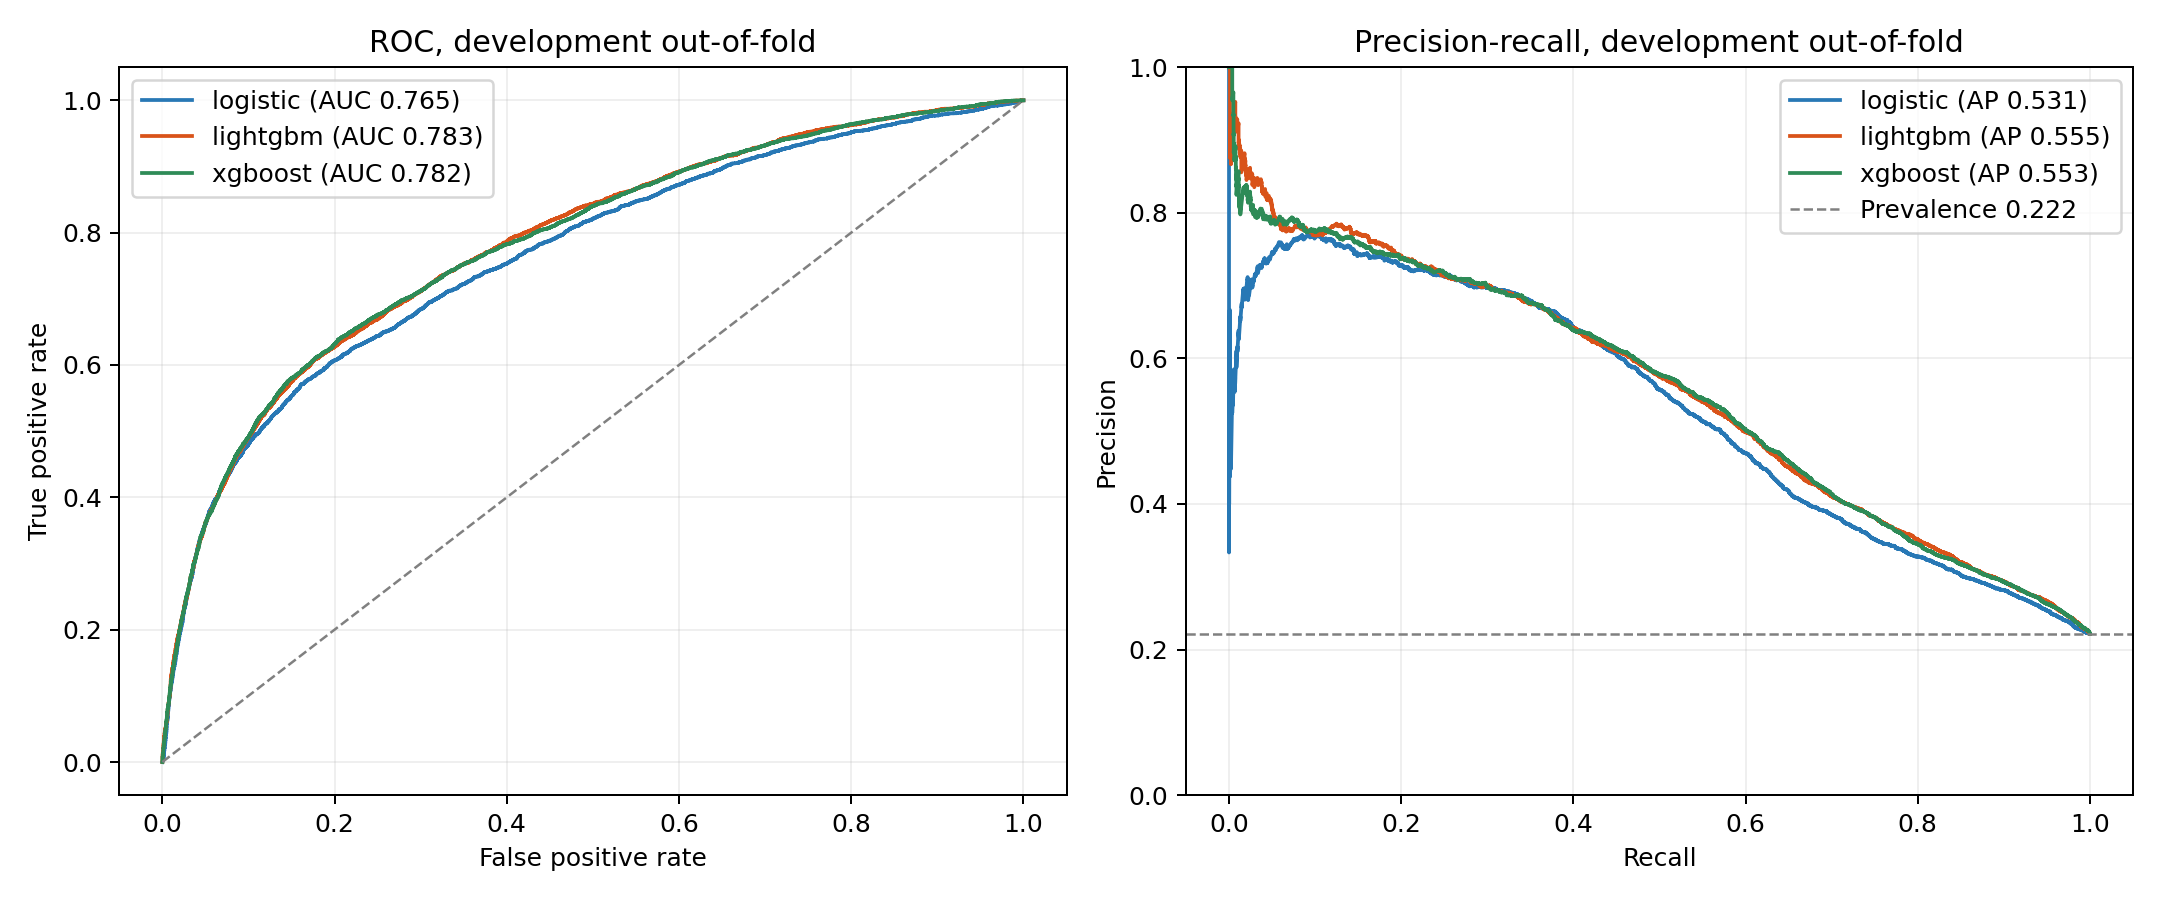
\includegraphics[width=0.95\linewidth]{t06_roc_pr_curves.png}
\caption{ROC and precision-recall curves from development OOF predictions.}
\end{figure}

\begin{figure}[ht]
\centering
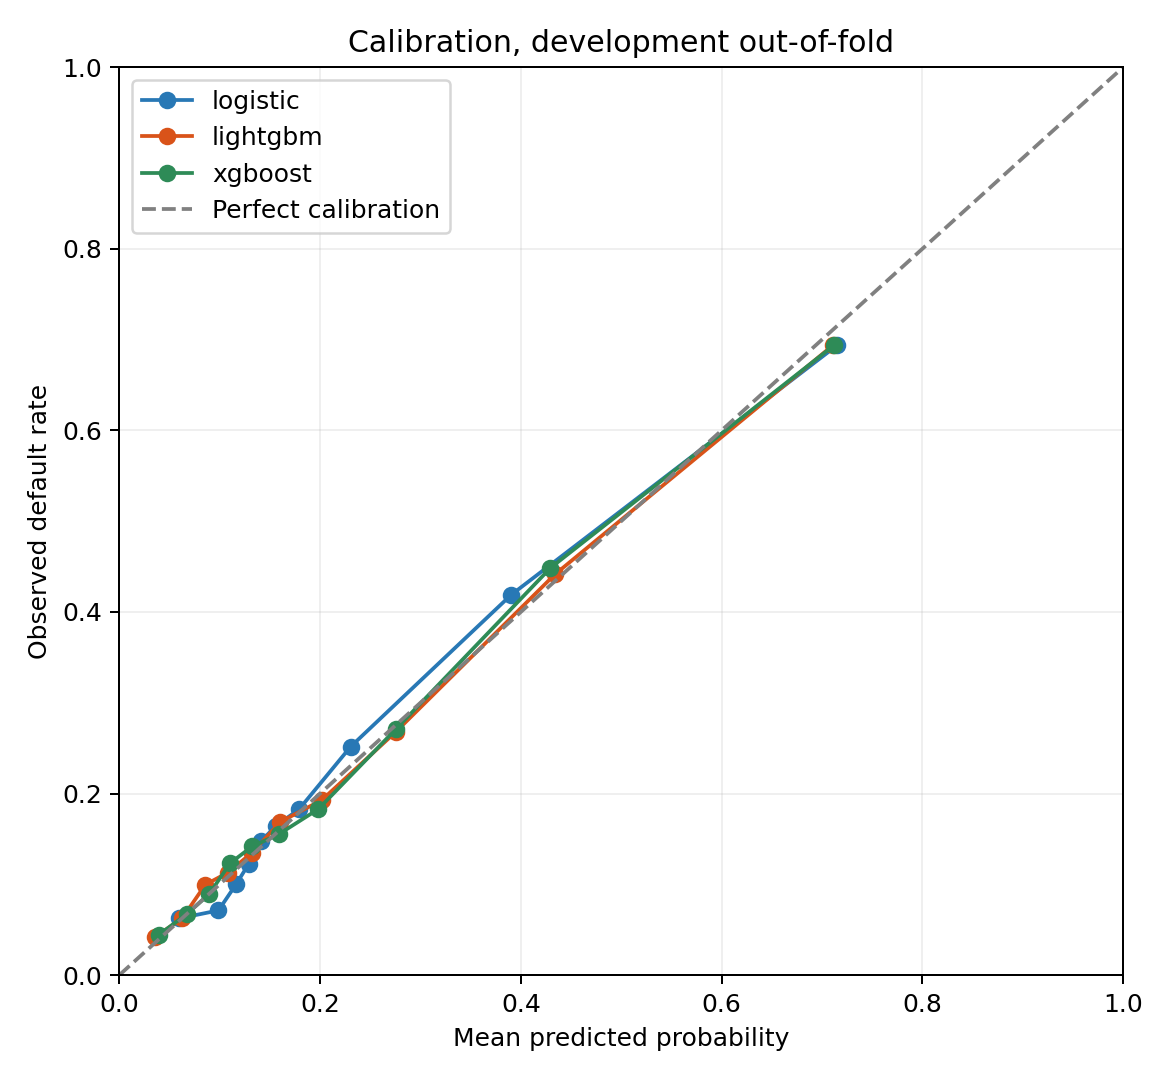
\includegraphics[width=0.82\linewidth]{t06_calibration_curve.png}
\caption{Calibration comparison from development OOF predictions.}
\end{figure}

\section{Feature screening and ablation}
The LightGBM null-importance task fits a model on each development training fold and compares actual gain shares with target-permuted fits. It uses 20 permutations per fold (100 null fits total), normalized gain importance, empirical upper-tail p-values with a plus-one correction, and Benjamini--Hochberg q-values. This is model-dependent screening evidence; its finite null sample limits p-value resolution, and it does not establish causality.

The ablation task evaluates the full feature set, each predeclared family alone, and each family removed, for logistic regression and LightGBM. Across both, removing repayment-status history had the largest effect. For LightGBM, AUC moved from 0.7829 to 0.7359 and average precision from 0.5547 to 0.4601 when those fields were removed. The isolated status-only LightGBM achieved AUC 0.7423 and average precision 0.5246. The difference between these diagnostic configurations can reflect redundancy and interactions; it is not a causal contribution or a final feature-selection policy.

\begin{figure}[ht]
\centering
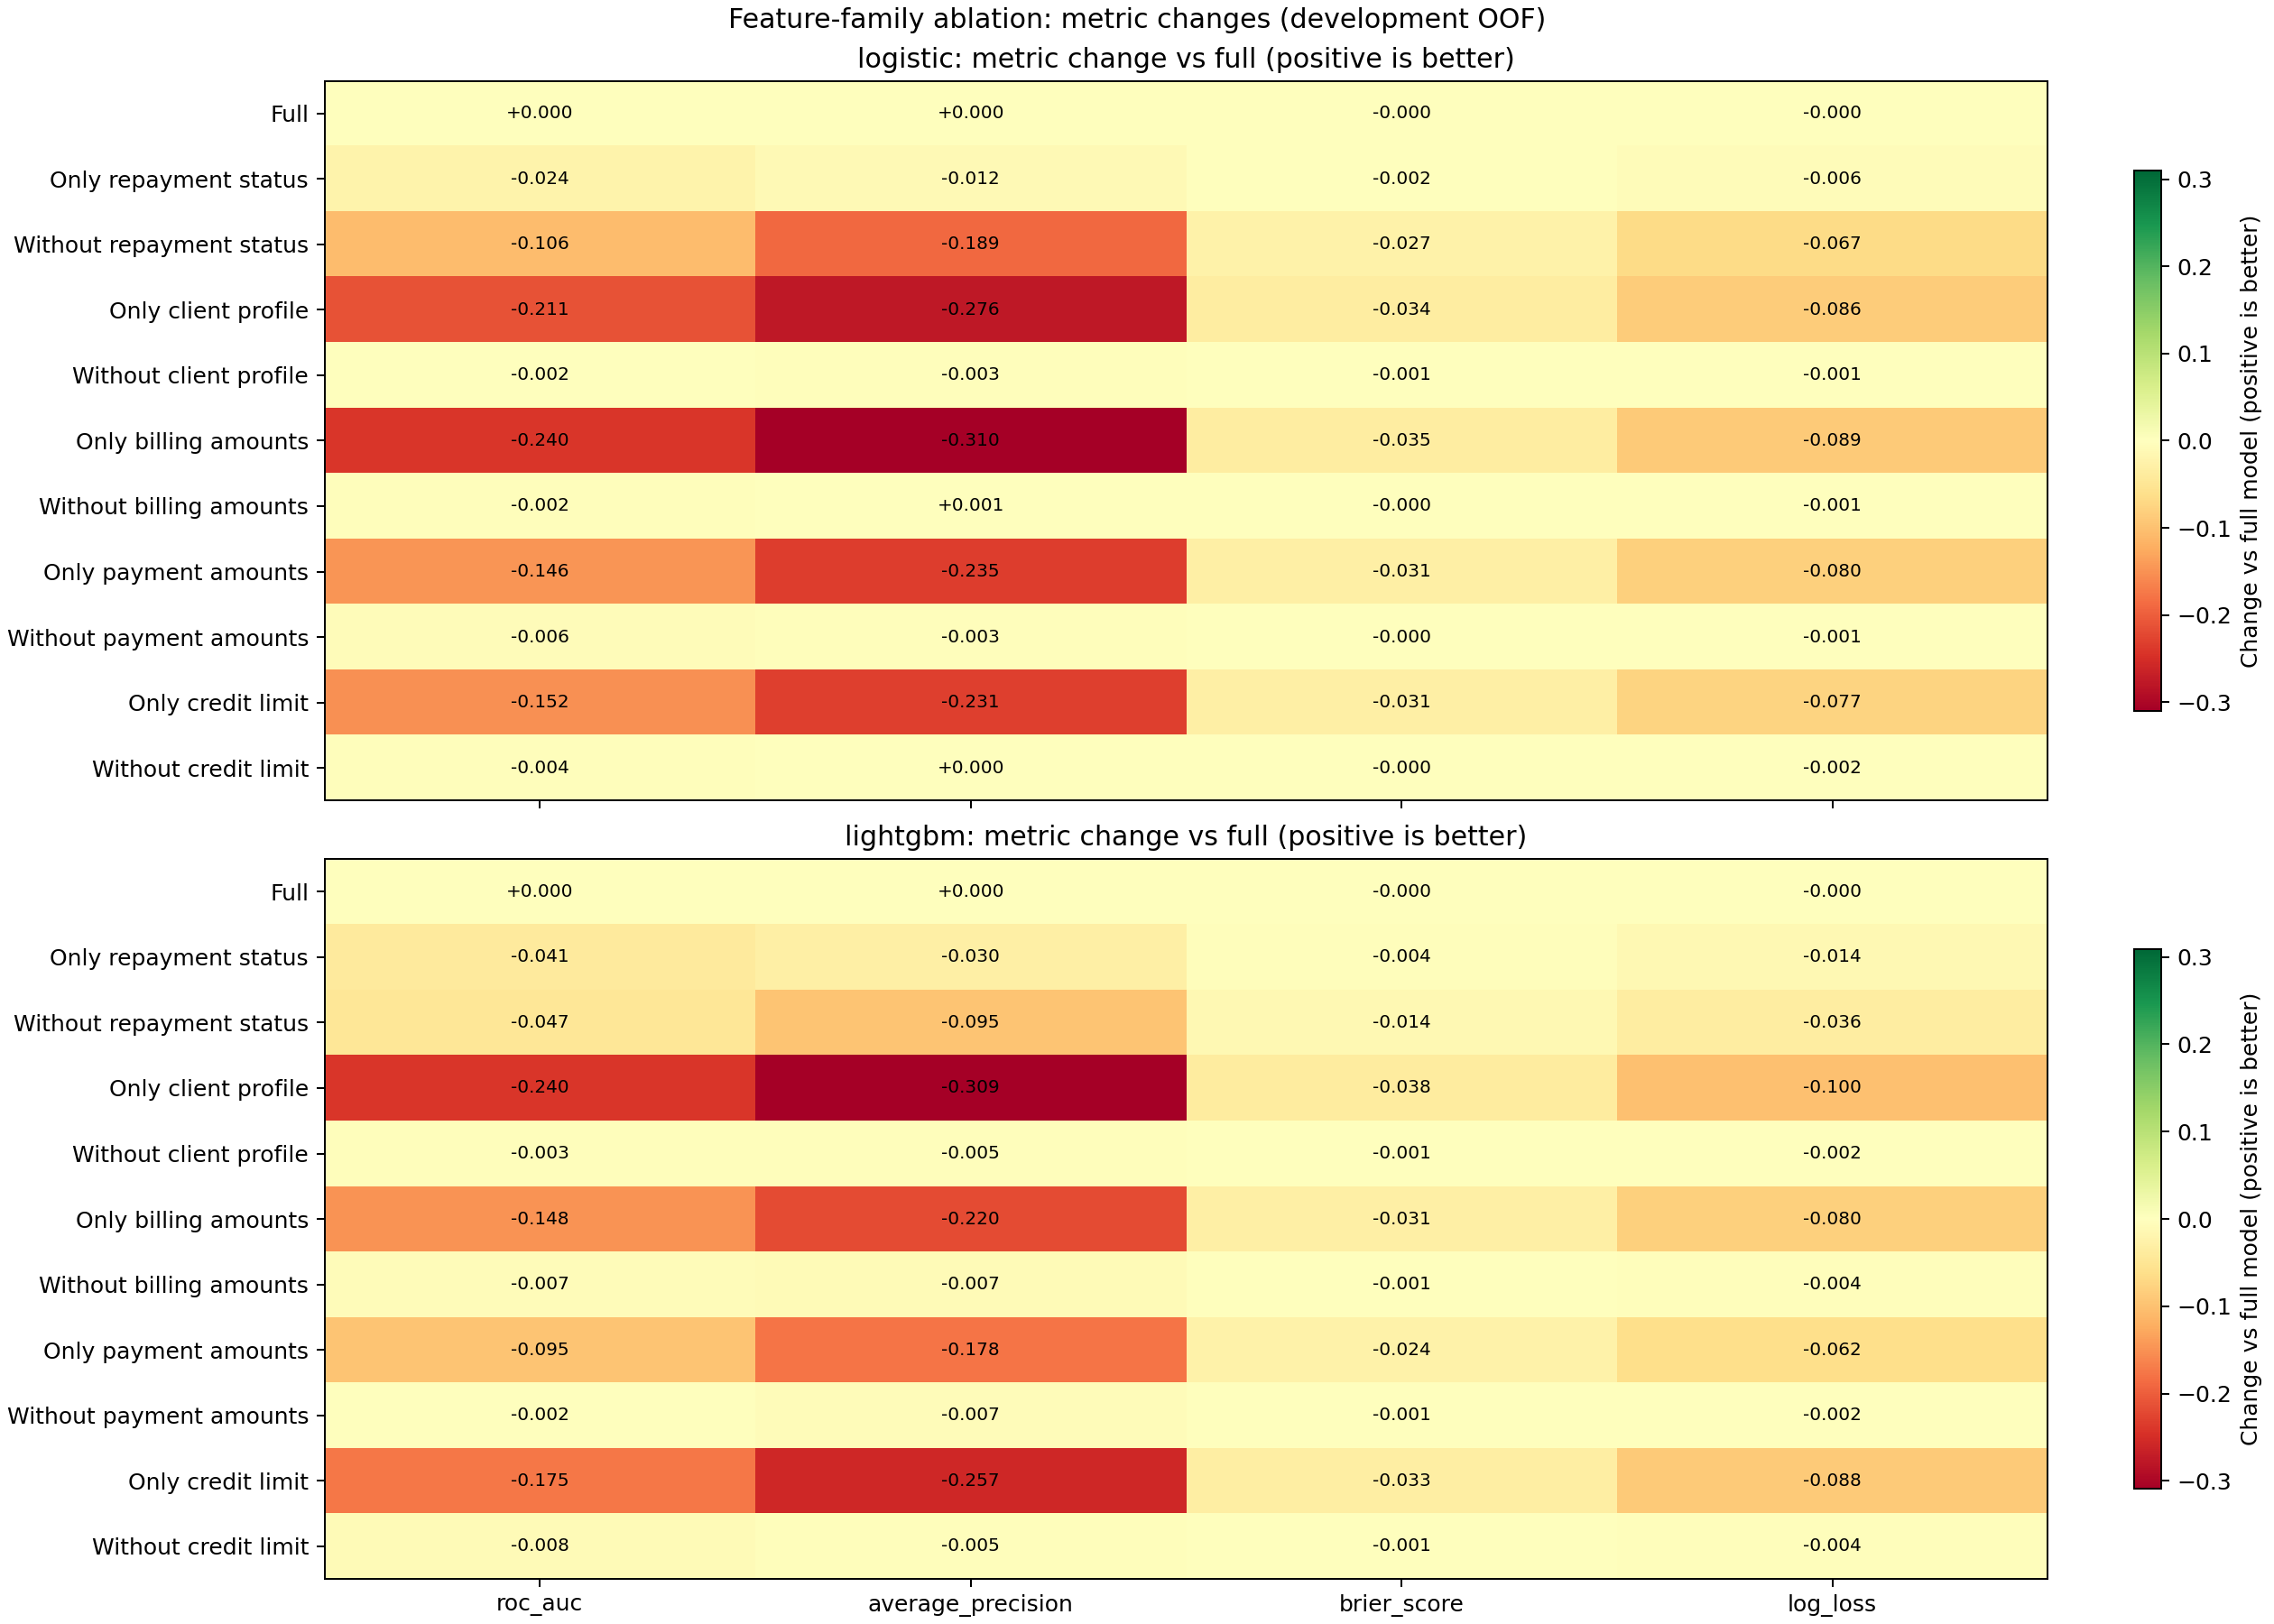
\includegraphics[width=0.9\linewidth]{t07_ablation_deltas.png}
\caption{Changes from the full feature set across the predeclared ablations.}
\end{figure}

\section{SQL mart and dashboard}
The analyst-facing app is `app/portfolio\_dashboard.py'. It loads the source workbook from a local path and registers client-level and normalized monthly-status tables in an in-memory DuckDB database. Its age and credit-limit controls update the KPI queries, status mix, transition table, and segment views. Reusable SQL is in `sql/portfolio\_mart.sql'; the aggregate export command is implemented in `scripts/build\_portfolio\_mart.py'.

The current unfiltered mart reconciles to 30,000 rows and 30,000 unique IDs. It reports a 22.12\% observed target mean, average stated limit of about 167,484, and median limit of 140,000 source currency units. The dashboard's September positive-code share is 22.7\%; this is explicitly `PAY\_0 > 0', not a broader delinquency or default rate. The six-month status chart counts client-month observations. The dashboard runs locally and does not write raw records or individual risk scores to the repository.

The practical use demonstrated is portfolio exploration and metric communication on a known historical sample. A real operational system would require a current, governed data feed; access controls; monitoring for missingness and schema changes; approved metric definitions; outcome and vintage monitoring; privacy and fairness review; documented ownership; and a business-approved action policy. None is supplied by this demo.

\section{Limitations and next steps}
\begin{itemize}
  \item One 2005 Taiwan vintage cannot test out-of-time drift or present-day portfolio performance.
  \item The outer test was deliberately locked and is not scored in this report. Reported metrics are development cross-validation estimates, not independent final-test estimates.
  \item Only one fixed configuration per model was compared; metrics and fold differences are descriptive, not a formal significance test.
  \item The group split prevents exact-profile overlap, but it does not solve sampling or temporal transportability.
  \item The target definition and measurement practices are historical; the dataset does not specify a deployable decision, intervention, or financial cost function.
  \item Demographic fields exist. No fairness assessment or protected-group decision analysis is presented here, and the dashboard does not expose those fields as operational filters.
  \item Dashboard filters enable descriptive analysis; segment gaps are neither causal effects nor recommended treatment rules.
\end{itemize}

Reasonable next steps are to conduct a decision-focused and fairness review, define a real monitoring contract with domain owners, and acquire appropriately licensed, current, representative data before assessing temporal validation. Do not tune a threshold or claim business value from the present evidence.

\section{Reproducible artifacts}
The detailed code map, environment instructions, and run commands are in \emph{Project Source Documentation}. Key evidence is saved under the T04--T07 result files and reports/portfolio\_mart/. Source checksum and split manifests are stored with the run metadata. The local source workbook is not bundled.

\section{Q\&A}
\textbf{Q: Is this model ready to make lending decisions?}\\
\textbf{A:} No. The evidence is offline, based on a single 2005 sample, and lacks current temporal validation, an operational target policy, fairness review, and business costs.

\textbf{Q: Which model won?}\\
\textbf{A:} LightGBM had the highest ROC AUC and average precision among the three fixed configurations, while XGBoost had slightly lower Brier score and log loss. Those small differences do not establish a general winner.

\textbf{Q: Why is there no score for the locked test set?}\\
\textbf{A:} It was reserved from model development and remains locked. The report avoids presenting a test score after choices were made on the development folds.

\textbf{Q: Why group duplicate profiles?}\\
\textbf{A:} The source contains repeated predictor profiles, including some with conflicting labels. Keeping each exact profile in one partition avoids optimistic validation from identical feature vectors on both sides.

\textbf{Q: What does the positive status-code share mean?}\\
\textbf{A:} It is the share of selected records with a positive numeric value in the latest source field `PAY\_0'. The dashboard does not equate it with a complete delinquency definition.

\textbf{Q: Can the dashboard be used on a company's portfolio?}\\
\textbf{A:} The code demonstrates a local analyst workflow, but real use requires an approved current data source, governed definitions, security controls, operational monitoring, and business review. Those steps are outside this public-data demonstration.

\textbf{Q: What would improve this project next?}\\
\textbf{A:} Use a representative multi-period dataset, define business actions and costs with stakeholders, test out-of-time performance, and complete fairness and decision-usefulness reviews before making any deployment proposal.

\vfill
\small\textbf{Primary source:} UCI Machine Learning Repository, \href{https://archive.ics.uci.edu/dataset/350/default+of+credit+card+clients}{Default of Credit Card Clients}, checked October 30, 2026. Dataset DOI: \href{https://doi.org/10.24432/C55S3H}{10.24432/C55S3H}.\par
\end{document}
